\documentclass[%
crop,%
tikz,%
convert={outext=.svg,command=\unexpanded{pdf2svg \infile\space../_static/\outfile}},%
multi=false%
]{standalone}%
\usepackage[utf8]{luainputenc}%
\usepackage[no-math]{fontspec}%
\defaultfontfeatures{%
    Numbers={OldStyle,Proportional},%
    Ligatures=TeX,%
    Extension=.ttf,%
}%
\setmainfont[%
UprightFont=*-Regular,%
ItalicFont=*-Italic,%
BoldFont=*-Bold,%
BoldItalicFont=*-BoldItalic,%
]{Raleway}%
\setsansfont[%
UprightFont=*-Regular,%
ItalicFont=*-Italic,%
BoldFont=*-Bold,%
BoldItalicFont=*-BoldItalic,%
]{Raleway}%
\usepackage[frenchmath]{mathastext}%
\usepackage{amsmath}%
\usepackage{amssymb}%
\usepackage{mathrsfs}%
\usepackage{mathtools}%
\usepackage{siunitx}%
\usepackage[siunitx]{circuitikz}%
\usetikzlibrary{calc,backgrounds,arrows.meta,patterns}%

\DeclareMathOperator{\sign}{sign}%

% Ensembles
\let\C\relax
\newcommand{\R}{\ensuremath{\mathbb{R}}} % Réel
\newcommand{\N}{\ensuremath{\mathbb{N}}} % Entiers naturels
% \newcommand{\C}{\ensuremath{\mathbb{C}}} % Complexes
\newcommand{\B}{\ensuremath{\mathscr{B}}} % Bus électriques
\newcommand{\Ch}{\ensuremath{\mathscr{C}}} % Charges
\renewcommand{\L}{\ensuremath{\mathscr{L}}} % Lignes
\renewcommand{\P}{\ensuremath{\mathscr{P}}} % Phases

% Phases
\newcommand{\arm}{\ensuremath{\mathrm{a}}}%
\newcommand{\brm}{\ensuremath{\mathrm{b}}}%
\newcommand{\crm}{\ensuremath{\mathrm{c}}}%
\newcommand{\nrm}{\ensuremath{\mathrm{n}}}%
\newcommand{\trm}{\ensuremath{\mathrm{t}}}%
\newcommand{\abrm}{\ensuremath{\mathrm{ab}}}%
\newcommand{\bcrm}{\ensuremath{\mathrm{bc}}}%
\newcommand{\carm}{\ensuremath{\mathrm{ca}}}%
\newcommand{\anrm}{\ensuremath{\mathrm{an}}}%
\newcommand{\bnrm}{\ensuremath{\mathrm{bn}}}%
\newcommand{\cnrm}{\ensuremath{\mathrm{cn}}}%
\newcommand{\atrm}{\ensuremath{\mathrm{at}}}%
\newcommand{\btrm}{\ensuremath{\mathrm{bt}}}%
\newcommand{\ctrm}{\ensuremath{\mathrm{ct}}}%
\newcommand{\ntrm}{\ensuremath{\mathrm{nt}}}%
\newcommand{\abcrm}{\ensuremath{\mathrm{abc}}}%
\newcommand{\abcnrm}{\ensuremath{\mathrm{abcn}}}%

% Indices ou exposants
\newcommand{\cons}{\ensuremath{\mathrm{cons.}}}%
\renewcommand{\prod}{\ensuremath{\mathrm{prod.}}}%
\newcommand{\theo}{\ensuremath{\mathrm{th.}}}%
\newcommand{\const}{\ensuremath{\mathrm{const.}}}%

% Variables
\newcommand{\umax}{\ensuremath{U^{\max}}}%
\newcommand{\umaxnorm}{\ensuremath{U^{\max\,\text{norm.}}}}%
\newcommand{\umin}{\ensuremath{U^{\min}}}%
\newcommand{\uminnorm}{\ensuremath{U^{\min\,\text{norm.}}}}%
\newcommand{\unom}{\ensuremath{U^{\text{nom.}}}}%
\newcommand{\unomnorm}{\ensuremath{U^{\text{nom.}\,\text{norm.}}}}%
\newcommand{\uup}{\ensuremath{U^{\text{up}}}}%
\newcommand{\uupnorm}{\ensuremath{U^{\text{up}\,\text{norm.}}}}%
\newcommand{\uupprime}{\ensuremath{U^{\text{up}\,\prime}}}%
\newcommand{\udown}{\ensuremath{U^{\text{down}}}}%
\newcommand{\udownnorm}{\ensuremath{U^{\text{down}\,\text{norm.}}}}%
\newcommand{\udownprime}{\ensuremath{U^{\text{down}\,\prime}}}%
\newcommand{\smax}{\ensuremath{S^{\max}}}%
\newcommand{\pmax}{\ensuremath{P^{\max}}}%
\newcommand{\sproj}{\ensuremath{\underline{S^{\text{proj.}}}}}%
%

\usepackage{pgfplots}%
\pgfplotsset{compat=newest}%

\begin{document}
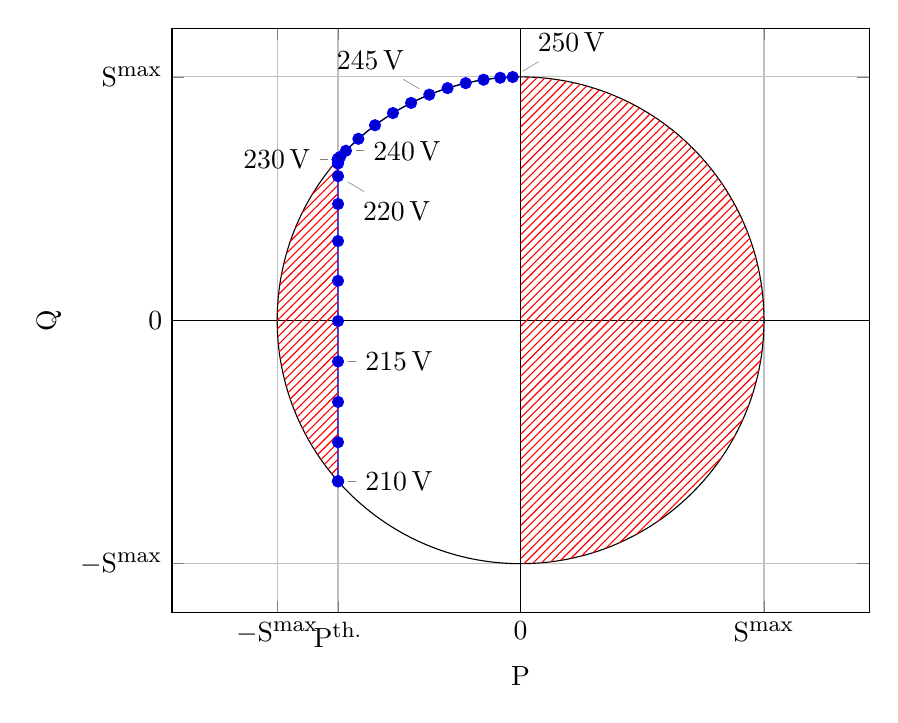
\begin{tikzpicture}[%
    show background rectangle,%
    tight background,%
    background rectangle/.style={fill=white}%
    ]
    %
    % Common parameters
    %
    % Control of P
    \pgfmathsetmacro{\umaxpvaleur}{250}%
    \pgfmathsetmacro{\umaxpnormvaleur}{1.0}%
    \pgfmathsetmacro{\uuppvaleur}{240}%
    \pgfmathsetmacro{\uuppnormvaleur}{\uuppvaleur/\umaxpvaleur}%
    \pgfmathsetmacro{\alphapvaleur}{400}%

    % Control of Q
    \pgfmathsetmacro{\umaxqvaleur}{240}%
    \pgfmathsetmacro{\umaxqnormvaleur}{1}%
    \pgfmathsetmacro{\uupqvaleur}{235}%
    \pgfmathsetmacro{\uupqnormvaleur}{\uupqvaleur/\umaxqvaleur}%
    \pgfmathsetmacro{\udownqvaleur}{220}%
    \pgfmathsetmacro{\udownqnormvaleur}{\udownqvaleur/\umaxqvaleur}%
    \pgfmathsetmacro{\uminqvaleur}{210}%
    \pgfmathsetmacro{\uminqnormvaleur}{\uminqvaleur/\umaxqvaleur}%
    \pgfmathsetmacro{\alphaqvaleur}{400}%


    % User-defined values
    \pgfmathsetmacro{\smaxvaleur}{5000}%
    \pgfmathsetmacro{\smaxnormvaleur}{1}%
    \pgfmathsetmacro{\pthvaleur}{3750}%
    \pgfmathsetmacro{\pthnormvaleur}{\pthvaleur/\smaxvaleur}%
    \pgfmathsetmacro{\angthvaleur}{acos(\pthvaleur/\smaxvaleur)}%
    \pgfmathsetmacro{\qthvaleur}{\smaxvaleur * sin(\angthvaleur)}%
    \pgfmathsetmacro{\qthnormvaleur}{\qthvaleur/\smaxvaleur}%

    %
    % Style
    %
    \tikzset{interdit/.style={pattern=north east lines, pattern color=red}}%

    \begin{axis}[%
        height=9cm,%
        % width=0.9\textwidth,%
        axis equal=true,%
        enlarge y limits,%
        enlarge x limits,%
        grid=major,%
        xmin=-\smaxnormvaleur,%
        xmax=\smaxnormvaleur,%
        ymin=-\smaxnormvaleur,%
        ymax=\smaxnormvaleur,%
        xlabel=$P$,%
        ylabel=$Q$,%
        xtick={-\smaxnormvaleur,-\pthnormvaleur,0,\smaxnormvaleur},%
        xticklabels={$-\smax$,$P^{\theo}$,0,$\smax$},%
        ytick={-\smaxnormvaleur,0,\smaxnormvaleur},%
        yticklabels={$-\smax$,0,$\smax$},%
        declare function={%
            fp(\t)=1.0+1.0/(\alphapvaleur*(\umaxpnormvaleur-\uuppnormvaleur)) *
            ln((1+exp(\alphapvaleur*(\t-\umaxpnormvaleur)))/(1+exp(\alphapvaleur*(\t-\uuppnormvaleur))));%
            p(\t)=-fp(\t/\umaxpvaleur)*\pthnormvaleur;%
            fq(\t)= 1.0/(\alphaqvaleur*(\uminqnormvaleur-\udownqnormvaleur)) *
            ln((1+exp(\alphaqvaleur*(\t-\udownqnormvaleur)))/(1+exp(\alphaqvaleur*(\t-\uminqnormvaleur))))-1.0;%
            gq(\t)=1.0/(\alphaqvaleur*(\umaxqnormvaleur-\uupqnormvaleur)) *
            ln((1+exp(\alphaqvaleur*(\t-\uupqnormvaleur)))/(1+exp(\alphaqvaleur*(\t-\umaxqnormvaleur))));%
            q(\t)=\qthnormvaleur +
            fq(\t/\umaxqvaleur)*(\smaxnormvaleur+\qthnormvaleur)+gq(\t/\umaxqvaleur)*(\smaxnormvaleur-\qthnormvaleur);%
            pclip(\t)=p(\t);%
            qclip(\t)=sign(q(\t))*sqrt(min(q(\t)^2,\smaxnormvaleur^2-p(\t)^2));%
        },%
        ]
        % Points
        \addplot+ [samples at={210,211,...,250}] ({pclip(\x)},{qclip(\x)});%

        % Cercle
        \draw (axis cs:0,0) circle[radius=\smaxnormvaleur];%

        % Axes
        \draw (axis cs:0,\pgfkeysvalueof{/pgfplots/ymin}) -- (axis
        cs:0,\pgfkeysvalueof{/pgfplots/ymax});%
        \draw (axis cs:\pgfkeysvalueof{/pgfplots/xmin},0) -- (axis
        cs:\pgfkeysvalueof{/pgfplots/xmax},0);%

        % Remplissage
        \fill[interdit] (axis cs:0,-\smaxnormvaleur) -- (axis cs:0,\smaxnormvaleur) arc[start
        angle=90, delta angle=-180, radius=\smaxnormvaleur];%
        \fill[interdit] (axis cs:-\pthnormvaleur,\qthnormvaleur) arc[start angle=180-\angthvaleur,
        delta angle=2*\angthvaleur, radius=\smaxnormvaleur];%

        %  Notes
        \node[pin={[pin distance=1mm] right:\SI{210}{\volt}}] at ({pclip(210)},{qclip(210)}) {};%
        \node[pin={[pin distance=1mm] right:\SI{215}{\volt}}] at ({pclip(215)},{qclip(215)}) {};%
        \node[pin={[pin distance=1mm] below right:\SI{220}{\volt}} ] at ({pclip(220)},{qclip(220)})
        {};%
        \node[pin={[pin distance=1mm] left:\SI{230}{\volt}} ] at ({pclip(230)},{qclip(230)}) {};%
        \node[pin={[pin distance=1mm] right:\SI{240}{\volt}}] at ({pclip(240)},{qclip(240)}) {};%
        \node[pin={[pin distance=1mm] above left:\SI{245}{\volt}}] at ({pclip(245)},{qclip(245)})
        {};%
        \node[pin={[pin distance=1mm] above right:\SI{250}{\volt}}] at ({pclip(250)},{qclip(250)})
        {};%
    \end{axis}
\end{tikzpicture}
\end{document}
% Local Variables:
% mode: latex
% TeX-engine: luatex
% TeX-source-correlate-method-active: synctex
% ispell-local-dictionary: "british"
% coding: utf-8
% LaTeX-indent-level: 4
% fill-column: 100
% End:
